\documentclass{beamer}
\mode<presentation> 


\usepackage{graphicx} % Allows including images

\begin{document}

\begin{frame}{Introduction}
\begin{itemize}
    \item  Finite Element Method (FEM) is a procedure of numerical solution of a domain viewed as the collection of sub-domains.
    \vspace{0.6cm}
    \item FEM on static structures computing the stress and displacement.
    \vspace{0.6cm}
    \item The actual problem will be replaced by simpler ones to find one approximate solution. 
\end{itemize}
    
\end{frame}


\begin{frame}{Gantt Chart : Progress}
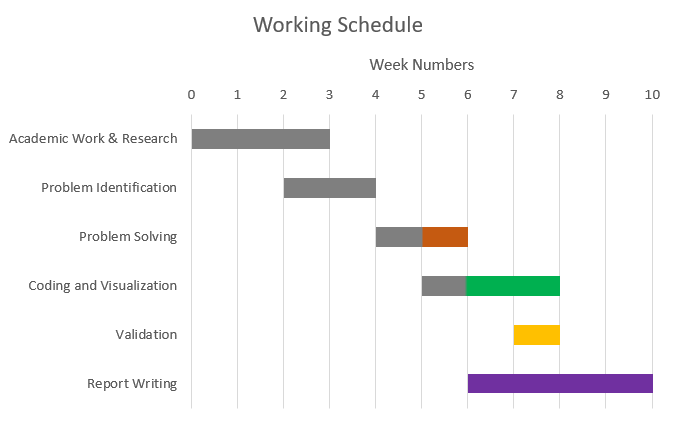
\includegraphics[width = 10cm, height = 6cm]{progress.png}
\end{frame}

\end{document}
